\chapter{Introduction}
\label{ch:introduction}
\section{Notations}
\label{sec:notations}
In this thesis, the following notations are used:
\begin{itemize}
  \item bold lowercase letters ($\vect{a}$, $\vect{b}$, $\vect{c}$) are used to denote vectors;
  \item italic lowercase letters ($a$, $b$, $c$) are used to denote scalars;
  \item bold uppercase letters ($\vect{A}$, $\vect{B}$, $\vect{C}$) are used to denote matrices;
  \item $\vect{a}_{i(j)}$ is the $j$th element of the vector $\vect{a}_i$;
  \item $||\vect{a}||_2$ is the $l^2$-norm of the vector $\vect{a}$, defined as $\sqrt{\sum_{i=1}^{n} a_i^2}$, denoted also as $\norm{a}$ for simplicity;
  \item $||\vect{a}||_n$ is the generic $l^n$-norm of the vector $\vect{a}$, defined as $\sqrt[n]{\sum_{i=1}^{n} \abs{a_i}^n}$;
  \item parenthesis encapsulating an index are used to condense descriptions, for example \quoted{\textbf{$\vect{a}_i(j)$ is the force applied to the $i$th ($j$th) step}} means that $\vect{a}_i$ is the force applied to the $i$th step and $\vect{a}_j$ is the force applied to the $j$th step;
\end{itemize}

No distinction in notation is made between a vector in the phisycal sense (applied to a point, with a direction, and a magnitude) and a vector in the mathematical sense (a generic number $\in \mathbb{R}^n $).

%\printinunitsof{in}\prntlen{\textwidth}

% \begin{figure*}
%   \centering
% \begin{subfigure}{0.3\linewidth}  % <----
%  % This file was created with tikzplotlib v0.10.1.
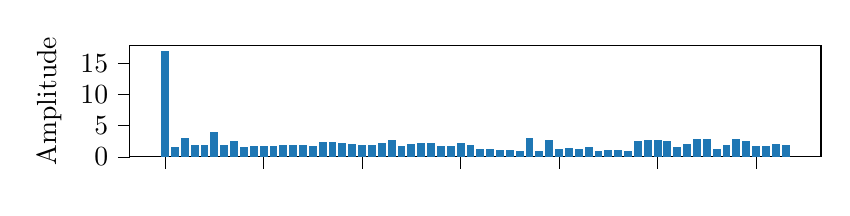
\begin{tikzpicture}

\definecolor{darkgray176}{RGB}{176,176,176}
\definecolor{steelblue31119180}{RGB}{31,119,180}

\begin{axis}[
height=3cm,
scaled x ticks=manual:{}{\pgfmathparse{#1}},
tick align=outside,
tick pos=left,
width=294.76926pt,
x grid style={darkgray176},
xmin=-3.59, xmax=66.59,
xtick style={color=black},
xticklabels={},
y grid style={darkgray176},
ylabel={Amplitude},
ymin=0, ymax=17.9224917606911,
ytick style={color=black},
ytick={0,5,10,15,20},
yticklabels={
  \(\displaystyle {0}\),
  \(\displaystyle {5}\),
  \(\displaystyle {10}\),
  \(\displaystyle {15}\),
  \(\displaystyle {20}\)
}
]
\draw[draw=none,fill=steelblue31119180] (axis cs:-0.4,0) rectangle (axis cs:0.4,17.0690397720867);
\draw[draw=none,fill=steelblue31119180] (axis cs:0.6,0) rectangle (axis cs:1.4,1.57701532870284);
\draw[draw=none,fill=steelblue31119180] (axis cs:1.6,0) rectangle (axis cs:2.4,3.04515592469192);
\draw[draw=none,fill=steelblue31119180] (axis cs:2.6,0) rectangle (axis cs:3.4,1.98727065046711);
\draw[draw=none,fill=steelblue31119180] (axis cs:3.6,0) rectangle (axis cs:4.4,1.87901229043815);
\draw[draw=none,fill=steelblue31119180] (axis cs:4.6,0) rectangle (axis cs:5.4,3.94494985947408);
\draw[draw=none,fill=steelblue31119180] (axis cs:5.6,0) rectangle (axis cs:6.4,1.94821362148988);
\draw[draw=none,fill=steelblue31119180] (axis cs:6.6,0) rectangle (axis cs:7.4,2.53456682074799);
\draw[draw=none,fill=steelblue31119180] (axis cs:7.6,0) rectangle (axis cs:8.4,1.53982779775888);
\draw[draw=none,fill=steelblue31119180] (axis cs:8.6,0) rectangle (axis cs:9.4,1.81855063876657);
\draw[draw=none,fill=steelblue31119180] (axis cs:9.6,0) rectangle (axis cs:10.4,1.74372106320514);
\draw[draw=none,fill=steelblue31119180] (axis cs:10.6,0) rectangle (axis cs:11.4,1.78981913351115);
\draw[draw=none,fill=steelblue31119180] (axis cs:11.6,0) rectangle (axis cs:12.4,1.9283565514217);
\draw[draw=none,fill=steelblue31119180] (axis cs:12.6,0) rectangle (axis cs:13.4,1.98727539890716);
\draw[draw=none,fill=steelblue31119180] (axis cs:13.6,0) rectangle (axis cs:14.4,1.83637697194901);
\draw[draw=none,fill=steelblue31119180] (axis cs:14.6,0) rectangle (axis cs:15.4,1.70629362470728);
\draw[draw=none,fill=steelblue31119180] (axis cs:15.6,0) rectangle (axis cs:16.4,2.32898911515285);
\draw[draw=none,fill=steelblue31119180] (axis cs:16.6,0) rectangle (axis cs:17.4,2.38726500121464);
\draw[draw=none,fill=steelblue31119180] (axis cs:17.6,0) rectangle (axis cs:18.4,2.2146470907513);
\draw[draw=none,fill=steelblue31119180] (axis cs:18.6,0) rectangle (axis cs:19.4,2.08886171015996);
\draw[draw=none,fill=steelblue31119180] (axis cs:19.6,0) rectangle (axis cs:20.4,1.91586717365543);
\draw[draw=none,fill=steelblue31119180] (axis cs:20.6,0) rectangle (axis cs:21.4,1.97741699428014);
\draw[draw=none,fill=steelblue31119180] (axis cs:21.6,0) rectangle (axis cs:22.4,2.26324345140917);
\draw[draw=none,fill=steelblue31119180] (axis cs:22.6,0) rectangle (axis cs:23.4,2.74150949309368);
\draw[draw=none,fill=steelblue31119180] (axis cs:23.6,0) rectangle (axis cs:24.4,1.67879784390802);
\draw[draw=none,fill=steelblue31119180] (axis cs:24.6,0) rectangle (axis cs:25.4,1.99560308046926);
\draw[draw=none,fill=steelblue31119180] (axis cs:25.6,0) rectangle (axis cs:26.4,2.18236194366914);
\draw[draw=none,fill=steelblue31119180] (axis cs:26.6,0) rectangle (axis cs:27.4,2.28116664486001);
\draw[draw=none,fill=steelblue31119180] (axis cs:27.6,0) rectangle (axis cs:28.4,1.76545125094874);
\draw[draw=none,fill=steelblue31119180] (axis cs:28.6,0) rectangle (axis cs:29.4,1.79936118428771);
\draw[draw=none,fill=steelblue31119180] (axis cs:29.6,0) rectangle (axis cs:30.4,2.21046386064049);
\draw[draw=none,fill=steelblue31119180] (axis cs:30.6,0) rectangle (axis cs:31.4,1.92512684988102);
\draw[draw=none,fill=steelblue31119180] (axis cs:31.6,0) rectangle (axis cs:32.4,1.29434219923151);
\draw[draw=none,fill=steelblue31119180] (axis cs:32.6,0) rectangle (axis cs:33.4,1.24905838096159);
\draw[draw=none,fill=steelblue31119180] (axis cs:33.6,0) rectangle (axis cs:34.4,1.0539404131426);
\draw[draw=none,fill=steelblue31119180] (axis cs:34.6,0) rectangle (axis cs:35.4,1.07785302549105);
\draw[draw=none,fill=steelblue31119180] (axis cs:35.6,0) rectangle (axis cs:36.4,1.00170991631713);
\draw[draw=none,fill=steelblue31119180] (axis cs:36.6,0) rectangle (axis cs:37.4,2.990570610034);
\draw[draw=none,fill=steelblue31119180] (axis cs:37.6,0) rectangle (axis cs:38.4,1.00976749017216);
\draw[draw=none,fill=steelblue31119180] (axis cs:38.6,0) rectangle (axis cs:39.4,2.77121989223762);
\draw[draw=none,fill=steelblue31119180] (axis cs:39.6,0) rectangle (axis cs:40.4,1.21267465980989);
\draw[draw=none,fill=steelblue31119180] (axis cs:40.6,0) rectangle (axis cs:41.4,1.44620941204964);
\draw[draw=none,fill=steelblue31119180] (axis cs:41.6,0) rectangle (axis cs:42.4,1.26138331095181);
\draw[draw=none,fill=steelblue31119180] (axis cs:42.6,0) rectangle (axis cs:43.4,1.60664374136418);
\draw[draw=none,fill=steelblue31119180] (axis cs:43.6,0) rectangle (axis cs:44.4,0.883196382772003);
\draw[draw=none,fill=steelblue31119180] (axis cs:44.6,0) rectangle (axis cs:45.4,1.0835546712407);
\draw[draw=none,fill=steelblue31119180] (axis cs:45.6,0) rectangle (axis cs:46.4,1.05267232084);
\draw[draw=none,fill=steelblue31119180] (axis cs:46.6,0) rectangle (axis cs:47.4,0.94061509525324);
\draw[draw=none,fill=steelblue31119180] (axis cs:47.6,0) rectangle (axis cs:48.4,2.5937245360833);
\draw[draw=none,fill=steelblue31119180] (axis cs:48.6,0) rectangle (axis cs:49.4,2.7964850933437);
\draw[draw=none,fill=steelblue31119180] (axis cs:49.6,0) rectangle (axis cs:50.4,2.71286149748853);
\draw[draw=none,fill=steelblue31119180] (axis cs:50.6,0) rectangle (axis cs:51.4,2.61834135486071);
\draw[draw=none,fill=steelblue31119180] (axis cs:51.6,0) rectangle (axis cs:52.4,1.64261763713365);
\draw[draw=none,fill=steelblue31119180] (axis cs:52.6,0) rectangle (axis cs:53.4,2.10765089952882);
\draw[draw=none,fill=steelblue31119180] (axis cs:53.6,0) rectangle (axis cs:54.4,2.79833649937833);
\draw[draw=none,fill=steelblue31119180] (axis cs:54.6,0) rectangle (axis cs:55.4,2.89223762573101);
\draw[draw=none,fill=steelblue31119180] (axis cs:55.6,0) rectangle (axis cs:56.4,1.32361974945306);
\draw[draw=none,fill=steelblue31119180] (axis cs:56.6,0) rectangle (axis cs:57.4,1.84030534558782);
\draw[draw=none,fill=steelblue31119180] (axis cs:57.6,0) rectangle (axis cs:58.4,2.82922380450697);
\draw[draw=none,fill=steelblue31119180] (axis cs:58.6,0) rectangle (axis cs:59.4,2.5822341294544);
\draw[draw=none,fill=steelblue31119180] (axis cs:59.6,0) rectangle (axis cs:60.4,1.71682916120663);
\draw[draw=none,fill=steelblue31119180] (axis cs:60.6,0) rectangle (axis cs:61.4,1.73398491114388);
\draw[draw=none,fill=steelblue31119180] (axis cs:61.6,0) rectangle (axis cs:62.4,2.13866133729592);
\draw[draw=none,fill=steelblue31119180] (axis cs:62.6,0) rectangle (axis cs:63.4,1.90570304888095);
\end{axis}

\end{tikzpicture}

%  \caption{Model 1}
%  \label{fig1a}
% \end{subfigure}

% \begin{subfigure}{0.3\linewidth}  % <----
%  % This file was created with tikzplotlib v0.10.1.
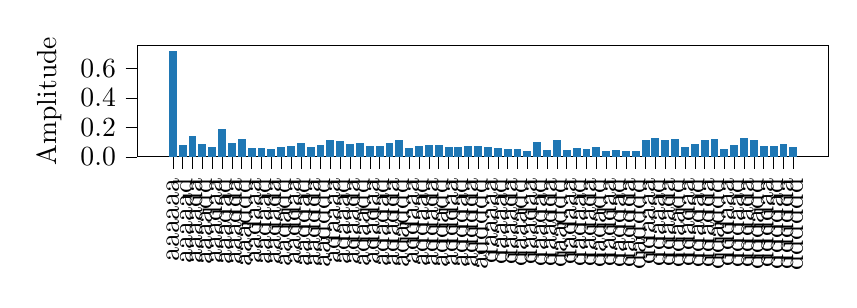
\begin{tikzpicture}

\definecolor{darkgray176}{RGB}{176,176,176}
\definecolor{steelblue31119180}{RGB}{31,119,180}

\begin{axis}[
height=3cm,
tick align=outside,
tick pos=left,
width=294.76926pt,
x grid style={darkgray176},
xmin=-3.59, xmax=66.59,
xtick style={color=black},
xtick={0,1,2,3,4,5,6,7,8,9,10,11,12,13,14,15,16,17,18,19,20,21,22,23,24,25,26,27,28,29,30,31,32,33,34,35,36,37,38,39,40,41,42,43,44,45,46,47,48,49,50,51,52,53,54,55,56,57,58,59,60,61,62,63},
xticklabel style={rotate=90.0},
xticklabels={
  aaaaaa,
  aaaaad,
  aaaada,
  aaaadd,
  aaadaa,
  aaadad,
  aaadda,
  aaaddd,
  aadaaa,
  aadaad,
  aadada,
  aadadd,
  aaddaa,
  aaddad,
  aaddda,
  aadddd,
  adaaaa,
  adaaad,
  adaada,
  adaadd,
  adadaa,
  adadad,
  adadda,
  adaddd,
  addaaa,
  addaad,
  addada,
  addadd,
  adddaa,
  adddad,
  adddda,
  addddd,
  daaaaa,
  daaaad,
  daaada,
  daaadd,
  daadaa,
  daadad,
  daadda,
  daaddd,
  dadaaa,
  dadaad,
  dadada,
  dadadd,
  daddaa,
  daddad,
  daddda,
  dadddd,
  ddaaaa,
  ddaaad,
  ddaada,
  ddaadd,
  ddadaa,
  ddadad,
  ddadda,
  ddaddd,
  dddaaa,
  dddaad,
  dddada,
  dddadd,
  ddddaa,
  ddddad,
  ddddda,
  dddddd
},
y grid style={darkgray176},
ylabel={Amplitude},
ymin=0, ymax=0.758179630791467,
ytick style={color=black},
ytick={0,0.2,0.4,0.6,0.8},
yticklabels={
  \(\displaystyle {0.0}\),
  \(\displaystyle {0.2}\),
  \(\displaystyle {0.4}\),
  \(\displaystyle {0.6}\),
  \(\displaystyle {0.8}\)
}
]
\draw[draw=none,fill=steelblue31119180] (axis cs:-0.4,0) rectangle (axis cs:0.4,0.722075838849016);
\draw[draw=none,fill=steelblue31119180] (axis cs:0.6,0) rectangle (axis cs:1.4,0.0816205118704516);
\draw[draw=none,fill=steelblue31119180] (axis cs:1.6,0) rectangle (axis cs:2.4,0.144788692125759);
\draw[draw=none,fill=steelblue31119180] (axis cs:2.6,0) rectangle (axis cs:3.4,0.0867045957893479);
\draw[draw=none,fill=steelblue31119180] (axis cs:3.6,0) rectangle (axis cs:4.4,0.0687644637243896);
\draw[draw=none,fill=steelblue31119180] (axis cs:4.6,0) rectangle (axis cs:5.4,0.191603550445973);
\draw[draw=none,fill=steelblue31119180] (axis cs:5.6,0) rectangle (axis cs:6.4,0.0912400814435433);
\draw[draw=none,fill=steelblue31119180] (axis cs:6.6,0) rectangle (axis cs:7.4,0.118441738979468);
\draw[draw=none,fill=steelblue31119180] (axis cs:7.6,0) rectangle (axis cs:8.4,0.063448949683056);
\draw[draw=none,fill=steelblue31119180] (axis cs:8.6,0) rectangle (axis cs:9.4,0.063549196660358);
\draw[draw=none,fill=steelblue31119180] (axis cs:9.6,0) rectangle (axis cs:10.4,0.0561566529115002);
\draw[draw=none,fill=steelblue31119180] (axis cs:10.6,0) rectangle (axis cs:11.4,0.0658459782078631);
\draw[draw=none,fill=steelblue31119180] (axis cs:11.6,0) rectangle (axis cs:12.4,0.0720379897131174);
\draw[draw=none,fill=steelblue31119180] (axis cs:12.6,0) rectangle (axis cs:13.4,0.0962993461770895);
\draw[draw=none,fill=steelblue31119180] (axis cs:13.6,0) rectangle (axis cs:14.4,0.0686195486369405);
\draw[draw=none,fill=steelblue31119180] (axis cs:14.6,0) rectangle (axis cs:15.4,0.0841955303823389);
\draw[draw=none,fill=steelblue31119180] (axis cs:15.6,0) rectangle (axis cs:16.4,0.114948175605847);
\draw[draw=none,fill=steelblue31119180] (axis cs:16.6,0) rectangle (axis cs:17.4,0.111103219250477);
\draw[draw=none,fill=steelblue31119180] (axis cs:17.6,0) rectangle (axis cs:18.4,0.0853474774953162);
\draw[draw=none,fill=steelblue31119180] (axis cs:18.6,0) rectangle (axis cs:19.4,0.0954229864952013);
\draw[draw=none,fill=steelblue31119180] (axis cs:19.6,0) rectangle (axis cs:20.4,0.0753330666191015);
\draw[draw=none,fill=steelblue31119180] (axis cs:20.6,0) rectangle (axis cs:21.4,0.0764573561609443);
\draw[draw=none,fill=steelblue31119180] (axis cs:21.6,0) rectangle (axis cs:22.4,0.0913486161286602);
\draw[draw=none,fill=steelblue31119180] (axis cs:22.6,0) rectangle (axis cs:23.4,0.115440781780618);
\draw[draw=none,fill=steelblue31119180] (axis cs:23.6,0) rectangle (axis cs:24.4,0.0605363919448476);
\draw[draw=none,fill=steelblue31119180] (axis cs:24.6,0) rectangle (axis cs:25.4,0.0715006546875076);
\draw[draw=none,fill=steelblue31119180] (axis cs:25.6,0) rectangle (axis cs:26.4,0.0834816059877538);
\draw[draw=none,fill=steelblue31119180] (axis cs:26.6,0) rectangle (axis cs:27.4,0.0825718187220844);
\draw[draw=none,fill=steelblue31119180] (axis cs:27.6,0) rectangle (axis cs:28.4,0.0657381299772261);
\draw[draw=none,fill=steelblue31119180] (axis cs:28.6,0) rectangle (axis cs:29.4,0.0684981211033183);
\draw[draw=none,fill=steelblue31119180] (axis cs:29.6,0) rectangle (axis cs:30.4,0.0735247581287173);
\draw[draw=none,fill=steelblue31119180] (axis cs:30.6,0) rectangle (axis cs:31.4,0.0714264975904106);
\draw[draw=none,fill=steelblue31119180] (axis cs:31.6,0) rectangle (axis cs:32.4,0.0674403501539547);
\draw[draw=none,fill=steelblue31119180] (axis cs:32.6,0) rectangle (axis cs:33.4,0.0592824747919798);
\draw[draw=none,fill=steelblue31119180] (axis cs:33.6,0) rectangle (axis cs:34.4,0.052030899559776);
\draw[draw=none,fill=steelblue31119180] (axis cs:34.6,0) rectangle (axis cs:35.4,0.0513258807665482);
\draw[draw=none,fill=steelblue31119180] (axis cs:35.6,0) rectangle (axis cs:36.4,0.0416017100177299);
\draw[draw=none,fill=steelblue31119180] (axis cs:36.6,0) rectangle (axis cs:37.4,0.101744455756126);
\draw[draw=none,fill=steelblue31119180] (axis cs:37.6,0) rectangle (axis cs:38.4,0.0463410493438625);
\draw[draw=none,fill=steelblue31119180] (axis cs:38.6,0) rectangle (axis cs:39.4,0.117328390407309);
\draw[draw=none,fill=steelblue31119180] (axis cs:39.6,0) rectangle (axis cs:40.4,0.0462494158731625);
\draw[draw=none,fill=steelblue31119180] (axis cs:40.6,0) rectangle (axis cs:41.4,0.0593257131667686);
\draw[draw=none,fill=steelblue31119180] (axis cs:41.6,0) rectangle (axis cs:42.4,0.0526934179057522);
\draw[draw=none,fill=steelblue31119180] (axis cs:42.6,0) rectangle (axis cs:43.4,0.0668781753176304);
\draw[draw=none,fill=steelblue31119180] (axis cs:43.6,0) rectangle (axis cs:44.4,0.0416416018534089);
\draw[draw=none,fill=steelblue31119180] (axis cs:44.6,0) rectangle (axis cs:45.4,0.0462760456257271);
\draw[draw=none,fill=steelblue31119180] (axis cs:45.6,0) rectangle (axis cs:46.4,0.0434239384103015);
\draw[draw=none,fill=steelblue31119180] (axis cs:46.6,0) rectangle (axis cs:47.4,0.0416410127228071);
\draw[draw=none,fill=steelblue31119180] (axis cs:47.6,0) rectangle (axis cs:48.4,0.117322919554115);
\draw[draw=none,fill=steelblue31119180] (axis cs:48.6,0) rectangle (axis cs:49.4,0.130187409367646);
\draw[draw=none,fill=steelblue31119180] (axis cs:49.6,0) rectangle (axis cs:50.4,0.114133627497582);
\draw[draw=none,fill=steelblue31119180] (axis cs:50.6,0) rectangle (axis cs:51.4,0.121358917513582);
\draw[draw=none,fill=steelblue31119180] (axis cs:51.6,0) rectangle (axis cs:52.4,0.0707478156876725);
\draw[draw=none,fill=steelblue31119180] (axis cs:52.6,0) rectangle (axis cs:53.4,0.0878711098289786);
\draw[draw=none,fill=steelblue31119180] (axis cs:53.6,0) rectangle (axis cs:54.4,0.112974228550204);
\draw[draw=none,fill=steelblue31119180] (axis cs:54.6,0) rectangle (axis cs:55.4,0.120443137445082);
\draw[draw=none,fill=steelblue31119180] (axis cs:55.6,0) rectangle (axis cs:56.4,0.053252675940857);
\draw[draw=none,fill=steelblue31119180] (axis cs:56.6,0) rectangle (axis cs:57.4,0.077975346334595);
\draw[draw=none,fill=steelblue31119180] (axis cs:57.6,0) rectangle (axis cs:58.4,0.125489421529731);
\draw[draw=none,fill=steelblue31119180] (axis cs:58.6,0) rectangle (axis cs:59.4,0.113761107750516);
\draw[draw=none,fill=steelblue31119180] (axis cs:59.6,0) rectangle (axis cs:60.4,0.0721800422035524);
\draw[draw=none,fill=steelblue31119180] (axis cs:60.6,0) rectangle (axis cs:61.4,0.0753054888730634);
\draw[draw=none,fill=steelblue31119180] (axis cs:61.6,0) rectangle (axis cs:62.4,0.0854419009187501);
\draw[draw=none,fill=steelblue31119180] (axis cs:62.6,0) rectangle (axis cs:63.4,0.0676569727174981);
\end{axis}

\end{tikzpicture}

%  \caption{Model 2}
%  \label{fig1b}
% \end{subfigure}

% \begin{subfigure}{0.3\linewidth}  % <----
%  % This file was created with tikzplotlib v0.10.1.
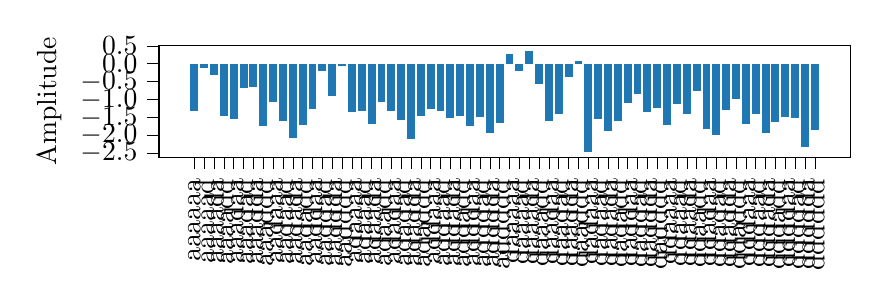
\begin{tikzpicture}

\definecolor{darkgray176}{RGB}{176,176,176}
\definecolor{steelblue31119180}{RGB}{31,119,180}

\begin{axis}[
height=3cm,
tick align=outside,
tick pos=left,
width=294.76926pt,
x grid style={darkgray176},
xmin=-3.59, xmax=66.59,
xtick style={color=black},
xtick={0,1,2,3,4,5,6,7,8,9,10,11,12,13,14,15,16,17,18,19,20,21,22,23,24,25,26,27,28,29,30,31,32,33,34,35,36,37,38,39,40,41,42,43,44,45,46,47,48,49,50,51,52,53,54,55,56,57,58,59,60,61,62,63},
xticklabel style={rotate=90.0},
xticklabels={
  aaaaaa,
  aaaaad,
  aaaada,
  aaaadd,
  aaadaa,
  aaadad,
  aaadda,
  aaaddd,
  aadaaa,
  aadaad,
  aadada,
  aadadd,
  aaddaa,
  aaddad,
  aaddda,
  aadddd,
  adaaaa,
  adaaad,
  adaada,
  adaadd,
  adadaa,
  adadad,
  adadda,
  adaddd,
  addaaa,
  addaad,
  addada,
  addadd,
  adddaa,
  adddad,
  adddda,
  addddd,
  daaaaa,
  daaaad,
  daaada,
  daaadd,
  daadaa,
  daadad,
  daadda,
  daaddd,
  dadaaa,
  dadaad,
  dadada,
  dadadd,
  daddaa,
  daddad,
  daddda,
  dadddd,
  ddaaaa,
  ddaaad,
  ddaada,
  ddaadd,
  ddadaa,
  ddadad,
  ddadda,
  ddaddd,
  dddaaa,
  dddaad,
  dddada,
  dddadd,
  ddddaa,
  ddddad,
  ddddda,
  dddddd
},
y grid style={darkgray176},
ylabel={Amplitude},
ymin=-2.61740256008719, ymax=0.509919465810349,
ytick style={color=black},
ytick={-3,-2.5,-2,-1.5,-1,-0.5,0,0.5,1},
yticklabels={
  \(\displaystyle {\ensuremath{-}3.0}\),
  \(\displaystyle {\ensuremath{-}2.5}\),
  \(\displaystyle {\ensuremath{-}2.0}\),
  \(\displaystyle {\ensuremath{-}1.5}\),
  \(\displaystyle {\ensuremath{-}1.0}\),
  \(\displaystyle {\ensuremath{-}0.5}\),
  \(\displaystyle {0.0}\),
  \(\displaystyle {0.5}\),
  \(\displaystyle {1.0}\)
}
]
\draw[draw=none,fill=steelblue31119180] (axis cs:-0.4,0) rectangle (axis cs:0.4,-1.31463451570886);
\draw[draw=none,fill=steelblue31119180] (axis cs:0.6,0) rectangle (axis cs:1.4,-0.134818691790791);
\draw[draw=none,fill=steelblue31119180] (axis cs:1.6,0) rectangle (axis cs:2.4,-0.319435036080992);
\draw[draw=none,fill=steelblue31119180] (axis cs:2.6,0) rectangle (axis cs:3.4,-1.45257985930736);
\draw[draw=none,fill=steelblue31119180] (axis cs:3.6,0) rectangle (axis cs:4.4,-1.5421469645371);
\draw[draw=none,fill=steelblue31119180] (axis cs:4.6,0) rectangle (axis cs:5.4,-0.673764853725896);
\draw[draw=none,fill=steelblue31119180] (axis cs:5.6,0) rectangle (axis cs:6.4,-0.651067231629759);
\draw[draw=none,fill=steelblue31119180] (axis cs:6.6,0) rectangle (axis cs:7.4,-1.74945636196658);
\draw[draw=none,fill=steelblue31119180] (axis cs:7.6,0) rectangle (axis cs:8.4,-1.07894447704247);
\draw[draw=none,fill=steelblue31119180] (axis cs:8.6,0) rectangle (axis cs:9.4,-1.611860529353);
\draw[draw=none,fill=steelblue31119180] (axis cs:9.6,0) rectangle (axis cs:10.4,-2.08587288612999);
\draw[draw=none,fill=steelblue31119180] (axis cs:10.6,0) rectangle (axis cs:11.4,-1.70951336361917);
\draw[draw=none,fill=steelblue31119180] (axis cs:11.6,0) rectangle (axis cs:12.4,-1.28157675228911);
\draw[draw=none,fill=steelblue31119180] (axis cs:12.6,0) rectangle (axis cs:13.4,-0.197861624149187);
\draw[draw=none,fill=steelblue31119180] (axis cs:13.6,0) rectangle (axis cs:14.4,-0.902246969989867);
\draw[draw=none,fill=steelblue31119180] (axis cs:14.6,0) rectangle (axis cs:15.4,-0.0599945188814577);
\draw[draw=none,fill=steelblue31119180] (axis cs:15.6,0) rectangle (axis cs:16.4,-1.36541350319367);
\draw[draw=none,fill=steelblue31119180] (axis cs:16.6,0) rectangle (axis cs:17.4,-1.3266188419031);
\draw[draw=none,fill=steelblue31119180] (axis cs:17.6,0) rectangle (axis cs:18.4,-1.69808295679741);
\draw[draw=none,fill=steelblue31119180] (axis cs:18.6,0) rectangle (axis cs:19.4,-1.08150865222734);
\draw[draw=none,fill=steelblue31119180] (axis cs:19.6,0) rectangle (axis cs:20.4,-1.3300365540605);
\draw[draw=none,fill=steelblue31119180] (axis cs:20.6,0) rectangle (axis cs:21.4,-1.56591194958796);
\draw[draw=none,fill=steelblue31119180] (axis cs:21.6,0) rectangle (axis cs:22.4,-2.10018255300044);
\draw[draw=none,fill=steelblue31119180] (axis cs:22.6,0) rectangle (axis cs:23.4,-1.46373211270423);
\draw[draw=none,fill=steelblue31119180] (axis cs:23.6,0) rectangle (axis cs:24.4,-1.27545670892696);
\draw[draw=none,fill=steelblue31119180] (axis cs:24.6,0) rectangle (axis cs:25.4,-1.33850245699865);
\draw[draw=none,fill=steelblue31119180] (axis cs:25.6,0) rectangle (axis cs:26.4,-1.52906230329855);
\draw[draw=none,fill=steelblue31119180] (axis cs:26.6,0) rectangle (axis cs:27.4,-1.45230662679311);
\draw[draw=none,fill=steelblue31119180] (axis cs:27.6,0) rectangle (axis cs:28.4,-1.73255965580102);
\draw[draw=none,fill=steelblue31119180] (axis cs:28.6,0) rectangle (axis cs:29.4,-1.50335007709024);
\draw[draw=none,fill=steelblue31119180] (axis cs:29.6,0) rectangle (axis cs:30.4,-1.94720337219532);
\draw[draw=none,fill=steelblue31119180] (axis cs:30.6,0) rectangle (axis cs:31.4,-1.65528675483821);
\draw[draw=none,fill=steelblue31119180] (axis cs:31.6,0) rectangle (axis cs:32.4,0.270054443767034);
\draw[draw=none,fill=steelblue31119180] (axis cs:32.6,0) rectangle (axis cs:33.4,-0.197751373312009);
\draw[draw=none,fill=steelblue31119180] (axis cs:33.6,0) rectangle (axis cs:34.4,0.367768464633188);
\draw[draw=none,fill=steelblue31119180] (axis cs:34.6,0) rectangle (axis cs:35.4,-0.564735648791296);
\draw[draw=none,fill=steelblue31119180] (axis cs:35.6,0) rectangle (axis cs:36.4,-1.61150252577791);
\draw[draw=none,fill=steelblue31119180] (axis cs:36.6,0) rectangle (axis cs:37.4,-1.40564010823609);
\draw[draw=none,fill=steelblue31119180] (axis cs:37.6,0) rectangle (axis cs:38.4,-0.371182760704031);
\draw[draw=none,fill=steelblue31119180] (axis cs:38.6,0) rectangle (axis cs:39.4,0.070349641149425);
\draw[draw=none,fill=steelblue31119180] (axis cs:39.6,0) rectangle (axis cs:40.4,-2.47525155891003);
\draw[draw=none,fill=steelblue31119180] (axis cs:40.6,0) rectangle (axis cs:41.4,-1.55614989351769);
\draw[draw=none,fill=steelblue31119180] (axis cs:41.6,0) rectangle (axis cs:42.4,-1.88234123808839);
\draw[draw=none,fill=steelblue31119180] (axis cs:42.6,0) rectangle (axis cs:43.4,-1.59270070771934);
\draw[draw=none,fill=steelblue31119180] (axis cs:43.6,0) rectangle (axis cs:44.4,-1.11190650381437);
\draw[draw=none,fill=steelblue31119180] (axis cs:44.6,0) rectangle (axis cs:45.4,-0.840681397994204);
\draw[draw=none,fill=steelblue31119180] (axis cs:45.6,0) rectangle (axis cs:46.4,-1.34368535787999);
\draw[draw=none,fill=steelblue31119180] (axis cs:46.6,0) rectangle (axis cs:47.4,-1.25517956985282);
\draw[draw=none,fill=steelblue31119180] (axis cs:47.6,0) rectangle (axis cs:48.4,-1.7101579930862);
\draw[draw=none,fill=steelblue31119180] (axis cs:48.6,0) rectangle (axis cs:49.4,-1.14244936083466);
\draw[draw=none,fill=steelblue31119180] (axis cs:49.6,0) rectangle (axis cs:50.4,-1.41050679464651);
\draw[draw=none,fill=steelblue31119180] (axis cs:50.6,0) rectangle (axis cs:51.4,-0.772205746905425);
\draw[draw=none,fill=steelblue31119180] (axis cs:51.6,0) rectangle (axis cs:52.4,-1.82325501180065);
\draw[draw=none,fill=steelblue31119180] (axis cs:52.6,0) rectangle (axis cs:53.4,-1.99315327974258);
\draw[draw=none,fill=steelblue31119180] (axis cs:53.6,0) rectangle (axis cs:54.4,-1.29641163379117);
\draw[draw=none,fill=steelblue31119180] (axis cs:54.6,0) rectangle (axis cs:55.4,-0.990550307115663);
\draw[draw=none,fill=steelblue31119180] (axis cs:55.6,0) rectangle (axis cs:56.4,-1.6980346169395);
\draw[draw=none,fill=steelblue31119180] (axis cs:56.6,0) rectangle (axis cs:57.4,-1.42284013393087);
\draw[draw=none,fill=steelblue31119180] (axis cs:57.6,0) rectangle (axis cs:58.4,-1.94315047574371);
\draw[draw=none,fill=steelblue31119180] (axis cs:58.6,0) rectangle (axis cs:59.4,-1.62789056222075);
\draw[draw=none,fill=steelblue31119180] (axis cs:59.6,0) rectangle (axis cs:60.4,-1.48520306606731);
\draw[draw=none,fill=steelblue31119180] (axis cs:60.6,0) rectangle (axis cs:61.4,-1.50855956912423);
\draw[draw=none,fill=steelblue31119180] (axis cs:61.6,0) rectangle (axis cs:62.4,-2.32843343387864);
\draw[draw=none,fill=steelblue31119180] (axis cs:62.6,0) rectangle (axis cs:63.4,-1.84413382243553);
\end{axis}

\end{tikzpicture}

%  \caption{Model 2}
%  \label{fig1b}
% \end{subfigure}

% \caption{Models}
% \label{fig2}
% \end{figure*}

% \begin{figure}[htbp]
%   \centering
%   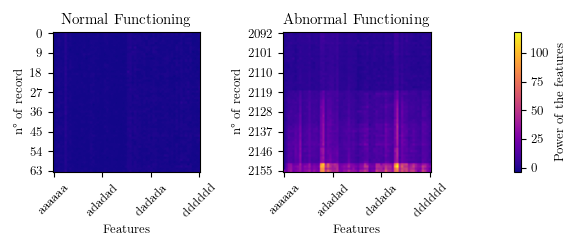
\includegraphics[scale=0.9]{images/Figure_5.png}
% \caption{Heatmap of the wavelet coefficients powers }
% \label{fig2}
% \end{figure}

% \begin{figure}[htbp]
%   \centering
%   \includesvg[width=\textwidth]{images/PMA_flowchart.svg}
% \caption{Predictive maintenance agent flowchart}
% \label{fig2}
% \end{figure}

% \begin{figure}[htbp]
%   \centering
%   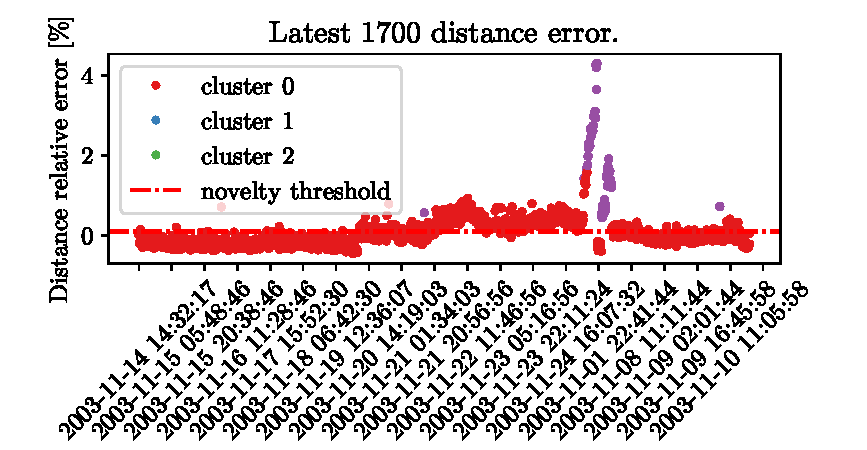
\includegraphics{images/Figure_1.pdf}
% \caption{Predictive maintenance agent flowchart}
% \label{fig2}
% \end{figure}